%*****************************************************
%	APPENDIX
%*****************************************************
\appendix

\chapter{Numerical modelling}

\section{Modelling of polar stochastic processes}
\label{app:modelling}
In this section,  an analysis of modelling techniques for the polar region is provided. Here, the focus is on developing models for Polar sea ice mechanics and dynamics. An overview of these models is given with a description of the variables and the scope of each model.

\subsection{Numerical modelling of sea ice}

The Hibler model is a numerical designed to investigate sea ice dynamics and thermodynamics in the Arctic region \cite{hibler1979dynamic}. This model attempts to couple the sea ice dynamics to Sea ice thickness and uses this relationship to investigate the relationship between the effects of sea ice and the climate. Work so far has largely studied these effects independently using factors that largely ignore the inherent mechanical properties of Sea Ice \cite{hibler1979dynamic}. Coupling these effects would allow for a more general descriptor of Sea Ice spread regions.\par

The model is based off \textcite{coon1974modeling} AIDJEX \cite{hibler1979dynamic}, who use plastic-elastic constitutive laws to describe large-scale sea Ice spreads. It is assumed that cracks, ridges, and leads are randomly distributed on large scales\footnote{100 km from \textcite{coon2007arctic}}. While the Hibler model is not as complex, it is more robust as it allows for larger time-steps and simplifies system boundaries. Here, sea ice is modelled using similar viscous plastic laws \cite{hibler1979dynamic} that allow for non-linear plastic flows to be modelled without severe limitations by large time-steps. The model uses the following components:

\begin{enumerate}
	\item    Momentum balance  - air and water stress
	\item    Coriolis force
	\item    Inertial forces
	\item    Constitutive laws - ice stress, strain, strength
	\item    Ice thickness distribution - accounting for open water patches, changes in thickness and Concentration
	\item    Ice strength 
\end{enumerate}
\begin{equation}
	\frac{mDu}{Dt} = -mfk\times u +\tau_a +\tau_w -mg \nabla H +F 
\end{equation}

$\frac{D}{Dt}$ is the substantial time derivative, k is a unit vector, u is the sea ice velocity, m is the ice mass, and f is the Coriolis parameter. Forces in the equation $\tau_a$, $\tau_w$ represent the respective stresses of the air and water. F is the force related to the internal ice stresses. H is the sea surface dynamic height, and g represents gravitational acceleration. Assuming constant turning angles, The air and water momentum equations are as follows
\begin{equation}
	\tau_a = \rho_a C_a|U_g|(U_g cos(\phi)+k\times U_g sin(\phi))
\end{equation}

\begin{equation}
	\tau_w = \rho_w C_w|U_w-u|[(U_w-u)cos(\phi)+k\times(U_w-u)sin(\phi)]
\end{equation}


where $\rho_a $ and $\rho_w$ are the densities of air and water, $C_a$/$C_w$ are the drag coefficients, $U_g$ is the geostrophic wind, and $U_w$ is the geostrophic ocean current\par

The Hibler model is the de facto numerical model for large scale ice process \cite{Rutgher2019SmallScale}. The model is used to describe an area of 10 - 100km$^2$. However, small scale models are still in development \cite{Rutgher2019SmallScale}.\par 

\subsubsection{Numerical modelling of ocean waves}
Ocean wave data is described by using spectral components with different magnitudes and wave periods. These spectral components are important in understanding the wave attenuation model \cite{williams2013wave} where, assuming the ice is modelled as a viscous fluid, wave energy is exponentially attenuated \cite{meylan2014situ}\cite{williams2013wave} with distance travelled into the ice due to partial reflections with the ice floes. The rate of attenuation is dependant on the wavelength. However, an exact mathematical relationship has not been found. The issue with verifying these models is the lack of robust data availability \cite{meylan2014situ}. Thereby reaffirming the need for increased in situ measurements.\par 

\textcite{williams2013wave} describe three fundamental components of Waves in Ice Modeling. These are advection, attenuation, and ice breakage \cite{williams2013wave}. Advection and attenuation describe how energy transfer occurs between waves and ice and are dependant on the group velocity $c_g$, and the attenuation factor $\hat{\alpha}$. These values are dependant on the frequency of the wave \cite{williams2013wave}. Also, the properties of ice are significant. These include Young's modulus $Y$, Poisson Ratio $\nu$, strain $\epsilon$ and viscous damping parameter $\Gamma$. Furthermore, the initial floe size distribution and sea ice concentration in a region are considered. The assumption is that wave breakage feeds back into the model with a new floe size distribution \cite{williams2013wave}. \par

Wave advection is described by the following energy model:
\begin{equation}
	\frac{1}{c_g}(\partial_t +c_g\partial_x)S(\omega;x,t) = R_{in}- R_{ice} - R_{other}- R_{nl}
\end{equation}
Where $R_{in}$ is the wind input energy, $R_{ice}$,$R_{nl}$,$R_{other}$ represent the energy loss from ice, other sources as well as non linear energy exchanges. $S(\omega;x,t)$ represents the waves in terms of its energy spectral density \cite{williams2013wave} For this model, the energy input is considered to come only from the rate of exchange between ocean and ice. Hence all other energy rates are considered 0 and $R_{ice}$ is defined in terms of $\hat{alpha} \text{ and } S$
\begin{equation}
	\frac{1}{c_g}(\partial_t +c_g\partial_x)S(\omega;x,t)  = -\hat{\alpha}(\omega,c,h,\langle D \rangle)S(\omega;x,t)
\end{equation}

$\hat{\alpha} = \frac{\alpha}{\langle D \rangle}$ describes the average attenuation per ice floe in terms of ice thickness and wave period \cite{williams2013wave}. By this definition, $R_ice$ is quasi linear \cite{williams2013wave} since a wave with a significantly large energy spectral density can break the floe decreasing the dimensions $\langle D \rangle$ and increase the dimensional attenuation factor $\hat{\alpha}$. The  operator $(\partial_t +c_g\partial_x)$ serves as the lagrangian reference fram at a moving velocity $c_g$. Finally, by breaking the above model into:
\begin{subequations}
	\begin{align}
		\frac{dx}{dt} = c_g(\omega,t_*,x) \label{advect}\\
		\frac{dS(\omega;x,t)}{dx} = -\hat{\alpha}(\omega,x,t_*,S_*)S(\omega;x,t) \label{atten}
	\end{align}
\end{subequations}

we can describe the dynamics of the sea ice during a breaking event at a time $t_*$  \cite{williams2013wave}. \par

The next step is determining the mathematical model for wave energy. A stochastic approach is taken to define key wave parameters \cite{williams2013wave}. The significant wave height is found using the formula
\begin{equation}
	H_s = 4\sqrt{m_0[n]}
\end{equation}
$m_n[\eta]$ describes the mean square surface sea elevation of a particle and is derived from the Spectral Density $S$ \cite{williams2013wave}.
\begin{equation}
	m_n[\eta] = \int_{0}{\infty}S(\omega)\omega^nd\omega
\end{equation}

The significant wave height can be considered four times the standard deviation of the surface elevation \cite{meylan2014situ}. Finally, by determining the significant wave height, the dominant wave period can be calculated as $\frac{1}{f_d}$ where $f_d$ is the frequency at which the dominant wave period occurs \cite{meylan2014situ}.

\section{ Modeling of GPS dilution of precision}
\label{appendix:GPS_DOP} 
Given a user's position on the earth, the distance from the user to the satellite is characterised by the following equation.
\begin{equation}
	r =  s - u
\end{equation}
where $r$ is the distance from the user to the satellite, $s$ is the distance from the earth's centre to the satellite and u is the distance from the earth to the user. By measuring the propagation time from the user to the satellite, The absolute distance $||r||$ can be calculated and hence, the pseudo-range can be calculated as
\begin{equation}
	\rho_i = ||s_i-u||+ct_b + v_{\rho_i}
\end{equation}
where $\rho_i$ is the pseudorange for satelite i, c is the speed of light, $t_b$ is  the clock offset and $v_{\rho_i}$ is the noise of the pseudorange measurement and:
\begin{equation}
	||s_i-u|| = \sqrt{(x_i - x_u)^2+(y_i-y_u)^2+(z_i-z_u)^2} \text{ for } i \in 1,2,3...N \label{los}
\end{equation}
where $N$ is the number of satellites and $(x_i,y_i,z_i)$ is the 3-dimensional position of satellite $i$. This represents a non-linear relationship for the line of sight from a receiver to a satellite.  \textcite{jwo2001efficient} explains that by creating a Taylor series centered on a nominal user position $(\hat{x_n},\hat{y_n},\hat{z_n})$ and ignoring the higher terms \cite{jwo2001efficient}. It then follows that:
\begin{equation}
	\Delta\rho_i = \rho_i - \hat{\rho_i} = e_{i1}\Delta x_u + e_{i2}\Delta x_u +  e_{i3}\Delta z_u
\end{equation}

The terms $e_{ij}$ represent the line of sight vector $E_i$ whereas the term $\hat{\rho_i}$ represennts the pseudo-range at the nominal user's position. It follows that the vector $E_i$ can be calculated as follows \cite{jwo2001efficient}.
\begin{subequations}
	\begin{align}
		e_{i1} = \frac{\hat{x_n} - x_i}{\hat{r_i}}\\
		e_{i2} = \frac{\hat{y_n} - y_i}{\hat{r_i}}\\
		e_{i3} = \frac{\hat{z_n} - z_i}{\hat{r_i}}\\
		\hat{r_i} = \sqrt{(\hat{x_n} - x_i)^2+(\hat{y_n} -y_i)^2+(\hat{z_n} -z_i)^2}
	\end{align}
\end{subequations}

Given $n$ satellites, the equation \eqref{los} can be written as a matrix with the following form:
\begin{equation}
	\textbf{z} = \textbf{Hx}+ \textbf{v}
\end{equation}
\begin{equation}
	\Delta \rho _i = \begin{bmatrix}
		\Delta \rho_1 &  \Delta \rho_2 &  \Delta \rho_3 & ... & \Delta \rho_n
	\end{bmatrix} 
\end{equation}
where 
\begin{subequations}
	\begin{align}
		\textbf{H} = \begin{bmatrix}
			e_{11} & e_{12} & e_{13}& 1 \\
			e_{21} & e_{22} & e_{23}& 1 
			\\
			e_{31} & e_{32} & e_{33}& 1
			\\
			... & ... & ... &  1 
			\\
			e_{n1} & e_{n2} & e_{n3} & 1
		\end{bmatrix}\\
		\textbf{x} = \begin{bmatrix}
			\Delta x_u \\ \Delta y_u \\\Delta z_u \\ c\Delta t_b
		\end{bmatrix}\\
		\textbf{v} = \begin{bmatrix}
			v_{\rho_1}\\
			v_{\rho_2}\\
			v_{\rho_3}\\
			...\\
			v_{\rho_n}
		\end{bmatrix}
	\end{align}
\end{subequations}

The matrix \textbf{H} is $n\times4$ where $n \geq 4$ to calculate all the parameters for GDOP \cite{jwo2001efficient}. We can then solve for the vector \textbf{x} by taking the psuedoinverse of H i.e $\hat{\textbf{x}} = (\textbf{H}^T\textbf{H})^{-1}\textbf{H}^t\textbf{z}$. Hence, given that the psuedorange is linearised, the quality of navigation is taken as the difference between the estimated position and the actual position \cite{jwo2001efficient}.
\begin{equation}
	\Tilde{\textbf{x}} = \hat{\textbf{x}} - x = (\textbf{H}^T\textbf{H})^{-1}\textbf{H}^Tv
\end{equation}
$E\{\Tilde{\textbf{x}}\Tilde{\textbf{x}}^T\}$ describes the covariance between the errors in the components of the estimated position \cite{jwo2001efficient} and is calculated as follows. 
\begin{equation}
	E\{\Tilde{\textbf{x}}\Tilde{\textbf{x}}^T\} = (\textbf{H}^T\textbf{H})^{-1}\textbf{H}^TE\{\textbf{vv}^T\} (\textbf{H}^T\textbf{H})^{-1}\textbf{H}
\end{equation}
Where $E\{\textbf{vv}^T\} = \sigma^2 I$. If all components of $\sigma$ are uncorrelated then the covariance become
\begin{equation}
	E\{\Tilde{\textbf{x}}\Tilde{\textbf{x}}^T\} = \sigma^2(\textbf{H}^T\textbf{H})^{-1}
\end{equation}
and thus the GDOP factor can be calculated from the RMS values of $\sigma^2$ i.e.
\begin{equation}
	GDOP = \frac{\sqrt{\sigma_{xx}^2+\sigma_{yy}^2+ \sigma_{zz}^2+\sigma_{tt}^2}}{\sigma}
\end{equation} where $\sigma_{xx}^2$,$\sigma_{yy}^2$,$\sigma_{zz}^2$,$\sigma_{tt}^2$ are the RMS values of the x,y and z time components respectively. THe value GDOP can also be decomposed into the positional dilution of precision (PDOP), time dilution of precision (TDOP), horizontal dilution of precision HDOP, and vertical dilution of precision (VDOP) which characterise the effects satellite spread on the 3-dimensional position, time, horizontal position and altitude respectively.\par

\section{Numerical techniques for modelling ocean waves}

\subsection{Kuik method}
\label{kuik}
The Kuik method is a computational technique used for measuring and determining the directional characteristics of ocean waves from the pitch and roll of an ocean buoy \cite{kuik1988method}. By using an accelerometer, gyroscope, or an inertial measurement system to measure the slope and heave of the three axes \cite{kuik1988method}, it is possible to reconstruct the sea state given a set of data of a specific length sampled above the Nyquist frequency of dominant ocean swells. A major advantage of the Kuik method is that the parameters are estimated directly from the Fourier transform of the measured signal \cite{kuik1988method} without assumptions about the measurement platform model. Therefore this technique can be applied to wave in ice measurements because no information is required about the dynamics of the model of the ice floe. This greatly improves the accuracy of the wave estimations since ice floes can vary in width, distribution and area as well as change shape due to collisions, freezing and melting. Wind waves are described using a two-dimensional energy spectrum $E$ with wave energy spread over a frequency $f$. The normalised distribution of energy over direction is defined according to \textcite{kuik1988method} as
\begin{equation}
	D_f(\theta) = \frac{E(f,\theta)}{\int_0^{2
			\pi}E(f,\theta)d\theta}
\end{equation} 

Finally, by computing the model per frequency, the distribution simplifies to $D(\theta)$ which can be approximated by a Fourier series with four terms \cite{kuik1988method} derived from the pitch, roll and heave of a buoy. Finally, the model can fully characterise the wave spectrum by calculating the following parameters from the Fourier coefficients:

\begin{enumerate}
	\item Mean wave direction $\theta_0$
	\item Directional width $\sigma$
	\item Skewness $\gamma$
	\item Kurtosis $\delta$ 
\end{enumerate}

The accuracy of the mean wave direction and width is affected by noise in the sampled data. small RMS values of noise can result in rapid increases of directional width by 1\% to 5\% \cite{kuik1988method}. Additionally, pitch and roll buoys are not free particles. They have an associated mass and, therefore, an associated inertia \cite{kuik1988method}. This results in a phase shift of the Fourier term by $\phi_i i \in {x,y,z}$  in the first harmonic \cite{kuik1988method}. This shift can result in an error of $0.5^\circ $ for $\sigma > 25 ^\circ $ to $1^\circ \text{ for } \sigma < 10^\circ $ \cite{kuik1988method}   

\subsection{Welch-Earle method}
\label{welchearl}
The Welch-Earle Method is an algorithm for calculating either directional and non-directional wave data depending on the assumptions of the input data \cite{earle1996nondirectional}. Data is derived from the vertical acceleration, and the roll and pitch of a buoy oriented perpendicular to the surface on either a vertically stabilised platform or a hull-fixed platform \cite{earle1996nondirectional}. Directional wave data is determined from both the acceleration, roll, pitch and heave from the buoy while non-directional wave data is calculated from time-series acceleration only. In this method, a digital time series representation of the vertical acceleration along with two orthogonal Gyroscope measurements and magnetometer readings relative to the earth’s magnetic field is obtained. This method accounts for the response function of the buoy. Thereby providing corrections to phase differences caused by the inertia of the buoy \cite{earle1996nondirectional}. Directional and non-directional wave data is characterised by calculating the spectra and co-spectra of discrete-time series data. The first part of the method was developed by \textcite{welch1967use} and is used to calculate the power spectral density.
Given a discrete time series data X(j) with a power spectral density P(f), |f|< $\frac{1}{2}$.this data segmented into a set of k-bins $X_k(j) | j \in {0,L-1}$ \cite{welch1967use}. Each bin is multiplied by a selected window function W(k) of length L. Additionally, bins are taken with a 50\% overlap to produce better statistical averages \cite{earle1996nondirectional} The Fast Fourier Transform (FFT) of the result is taken to for a periodograms $I_k$ \cite{earle1996nondirectional}. Finally, the new power spectral estimator $\hat{P}(f_n)$ is calculated by taking the average of the K periodograms as shown in \textcite{welch1967use}

\begin{equation}
	\hat{P}(f_n) = \frac{1}{K}\sum^K_{k=1}I_k(f_n)
\end{equation}

where 
\begin{equation}
	f_n = \frac{n}{L} | n \in 0,1,2... \frac{L}{2}
\end{equation}

Detrending is used to account for the effects of buoy motion on the time series. The inertia of the platform results in non-zero mean trends often as a result of constant wind or currents acting on the hull of the buoy \cite{earle1996nondirectional}. These must be discarded before the spectrum and co spectra are calculated. The resolution of the accelerometer is important for accurately tracking acceleration \cite{kohout2015device}. If the resolution is too small, low accelerations will not be recorded resulting in incorrect vertical accelerations being calculated. \textcite{kohout2015device} found that a low-resolution IMU was unable to reliably flag that it had exceeded a boundary condition and hence it was discarded \cite{kohout2015device}.\par 

The spectra and co-spectra of the directional and non-directional wave series can be calculated by computing the spectrum $S(x)$ as a function of frequency and direction (as is similar to the Kuik method). \textcite{earle1996nondirectional} show that characterisation of the co-spectra $C(x)$ and spectrum$S(x)$ can be achieved by calculating the first four Fourier coefficients. Finally, the sea state can be represented by calculating the following parameters

\begin{enumerate}
	\item Longuet-Higgins directional parameters
	\begin{enumerate}
		\item $a_0$
		\item $a_1$
		\item $b_0$
		\item $b_1$
	\end{enumerate}
	\item Significant wave height $H_0$
	\item Dominant wave period $T_p$
	\item Total degrees of freedom $TDF$
	\item Average zero-crossing period $T_{av}$
	\item Zero-crossing period $T_{zero}$
\end{enumerate}

This approach brings into account the possibility of spectral leakage however, this can be greatly minimised by sampling above the Nyquist frequency of the upper Wave frequency band (generally taken to be 0.5Hz) for a minimum of 1000 seconds (about 16 – 17 minutes). Additionally, spectral leakage can be reduced by selecting a window function with a gradual taper such as a half cosine or Hanning taper \cite{welch1967use}\par

\section{Temperature sensing measurement techniques}
\label{appendix:tempsense}
\subsubsection{Thermistors}

Modern thermistors have progressed significantly in the past decade. Until recently, they had been considered inaccurate with uncertainty ranges of up to 5\% \cite{tong2001improving}. Thermistors are capable of providing accuracies of up to 0.01$^\circ$ C. They consist of a semiconductor that changes its resistance in response to temperature \cite{childs2000review}. They have a faster response time than their resistive counterpart: the resistive temperature detector (RTD) which, works on the same principle for temperature measurement. However, where RTDs have a positive temperature coefficient, thermistors have a negative temperature coefficient \cite{tong2001improving}. These devices can operate over a substantial, albeit relatively limited, range of $-100^\circ - 300^\circ C$. The major trade-off with these devices is the lack of standards \cite{tong2001improving}. Operating the device involves a large degree of uncertainty. Also, these devices are not powerful enough to accurately reach the desired ranges alone and require additional circuits. Finally, the response curve is nonlinear. The  relationship between resistance and temperature is \cite{childs2000review}:
\begin{equation}
	R_T = R_0e^{1 - B(\frac{1}{T}- \frac{1}{T_0})}
\end{equation}
where $R_T$ is the temperature measured, $R_0$ is the resistance at a known temperature of $T_0$, T is the temperature, and B is a coefficient based on the inherent properties of the thermistor. Finally, these devices are more prone to noise from excitation current.

\subsubsection{Silicon temperature devices}

Semiconductor temperature devices (STDs) are suited to applications where the temperature ranges from -55 to 150 $^\circ$ C. These devices provide a stable output with a typical accuracy of $0.8 ^\circ $ C. These devices typically consist of diodes and transistors with a bandgap voltage that changes with a change in temperature \cite{childs2000review}. STDs are advantageous in electronic application due to their small form, high accuracy and stability. These devices are relatively simple and have a good sensitivity to changes \cite{childs2000review}. Diodes are typically used in semiconductor devices. Here, the forward voltage drop across the p-n junction is linearly proportional to the Ambient temperature over a certain temperature range (typically 25K - 400K) \cite{childs2000review}. These devices consist of either silicon or Gallium-Arsenide. Silicon is preferred as it has better stability at low temperatures and is cheaper. However, this comes at the trade-off of a lower voltage output \cite{childs2000review}. \par These types of devices are readily available in integrated circuit (IC) forms and are manufactured in a variety of packages, types and compositions for any application. Typical devices are DS18B20, LM355 or BMP2080. Recent innovations in Silicon sensing have seen the rise of CMOS devices and Micro Electrical-Mechanical Systems (MEMS) used more frequently \cite{mansoor2015silicon}. While these devices can suffer from deterioration due to self-heating, \textcite{mansoor2015silicon} discuss that the low-power operation of these devices can offset this issue which is advantageous for systems that constrained by power consumption. However, a major disadvantage with these devices is that STDs work ideally with a purely DC signal as an AC coupled signal can cause significant errors in the output \cite{childs2000review} \cite{mansoor2015silicon}. These errors can be the result of improper shielding and poor grounding. Hence proper shielding and grounding are required to reduce these errors. Finally, these devices require careful calibration before use.

\section{Pressure sensing techniques}
\subsubsection{Diaphragm based sensors}

The current state of pressure sensing technology is driven towards the miniature MEMs version of large scale devices \cite{eaton1997micromachined}. Most large scale pressure sensors consist of a diaphragm mounted on a device in a known way. The diaphragm is coupled to a device that converts the pressure to a mechanical movement which is then measured using a gauge. These senses often had a secondary sensor that converts the mechanical movement to an electrical signal which is measured \cite{eaton1997micromachined}. These sensors determine pressure by measuring the deflection of a miniature diaphragm. This deflection is converted to an electrical signal. Typically, a reference pressure is provided as a measurement of a sealed chamber or absolute pressure port. Assuming the simplest version of this sensor i.e. a plate of uniform thickness \cite{eaton1997micromachined} The deflection $w$ of the diaphragm is related to the pressure  $P$ by the following equation: \cite{eaton1997micromachined}

\begin{equation}
	w(r) = \frac{Pa^4}{64D}(1- (\frac{r}{a})^2)^2
\end{equation}

where r is the deformed radius of the diaphragm, a is the original radius and D is the  rigidity of the diaphragm governed by the equation:

\begin{equation}
	D = \frac{Eh^3}{12(1-v^2)}
\end{equation}
where E,h,v are Young's modulus, thickness and Poisson's ratio of the disc \cite{eaton1997micromachined}. This technique suffers from a multitude of problems. The diaphragm is susceptible to plastic deformation, while more robust diaphragms result in more complex relationships. The current relationship is nonlinear and can result in calculation errors. Eaten (1997) advocate for the use of MEMs based electronics on these principles.

\subsubsection{Piezoresistive sensors}

Piezoresistive sensors are electric devices constructed out of a semiconductor whose electrical properties change when stress is applied \cite{eaton1997micromachined}. These devices are mounted to a diaphragm and exhibit a linear change in resistance with a change in [ressure. Currently, these sensors take the form of single-crystal diaphragms with piezoelectric resistors diffused through the materials. The advantage of these devices is robustness towards hysteresis and measurement drift. At low temperatures, silicon exhibits near-perfect elastic behaviour and is three times the tensile strength of strain gauges\cite{eaton1997micromachined}. However, these sensors are susceptible to thermal expansion resulting in temperature measurement drift \cite{samaun1971ic}. Additionally, these sensors require resistors with identical temperature resistance characteristics, or the pressure measurement will be inaccurate. Finally, compensation techniques are required to calibrate the accuracy of the sensor.

\subsubsection{Capacitive sensors}

These sensors consist of parallel conductive plates. Assuming a constant, known dielectric, an external pressure causes the plates to deform which changes the capacitance C according to the relationship \cite{eaton1997micromachined}
\begin{equation}
	C = \int \int \frac{\epsilon}{d - w(r)}drd\theta
\end{equation}

Where $w(r)$ is the deformation of the plate, $\epsilon$ is the strain experienced by the plate, and d is the distance of separation. The pressure capacitance relationship can be approximated using a least-squares fit \cite{eaton1997micromachined}. However, this results in model errors of 1.5\% and up to 11\% at $w = \frac{1}{2}h$ for the plate height. These sensors are more advantageous over piezoresistive sensors as they have higher pressure sensitivity and reduced susceptibility to temperature drift. However, these sensors are significantly susceptible to parasitic capacitance, which can result in losses and errors. Additionally, these sensors are simple in design. However, they tend towards more complex circuit requirements.

\newpage
\chapter{Project design}

\section{Stakeholder analysis}
\label{app:stakeholder}
For this project, a stakeholder is defined as any user or set of users who will impact the overall project or be impacted by the final design of the project \cite{varvasovszky2000stakeholder}. The stakeholders for this project can be considered as an individual directly involved in the designing/building of the project or a user: i.e. an individual responsible for using the system or any data it generates.  These project stakeholders are shown in Table \ref{tab:stake}.

\begin{table}[H]
	\centering
	\caption{Table showing the key stakeholders in the project, their level of involvement as well as their interests in the project.}
	\label{tab:stake}
	\setlength{\extrarowheight}{5pt}
	\resizebox{\textwidth}{!}{%
		\begin{tabular}{  >{\RaggedRight}m{0.3\textwidth}  >{\RaggedRight}m{0.4\textwidth} >{\RaggedRight}m{0.4\textwidth}  }
			\hline
			\textbf{Stakeholder} &  \textbf{Function} & \textbf{Involvement}\\
			\hline
			\hline
			Lead scientist \hfill & Principal stakeholder: Initiates and funds the SHARC buoy project. & Sets the user requirements, provides feedback on progress, organises expeditions.  \\
			\hline
			Project supervisor & Set the project timeline and provide feedback on progress.\hfill& Primary engagement with principle stakeholder.\\
			\hline
			Project engineer & Translate specifications to subsystems. & Selecting hardware, sourcing materials as well as designing firmware for the buoy. \\
			\hline
			Deployment team & Place the system in a selected location and ensure the device is communicating & Physical handling of the device, understanding how the system works.\\
			\hline
			User & Collect and archive data packets from the buoy. & Interact with the data portal and decompression software.\\
			\hline
			Collaborators & Work with users on interpreting data from the system. & Analysing generated data sets.\\
			\hline
			\hline
	\end{tabular}}
\end{table}

\section{Acceptance test protocols}
\label{app:atp}


\begin{table}[H]
	\centering
	\caption{Acceptance test protocol for subsystem connectivity testing.}
	\setlength{\extrarowheight}{5pt}
	\resizebox{\textwidth}{!}{%
		\begin{tabular}{|>{\raggedright\arraybackslash}m{0.25\textwidth}|>{\raggedright\arraybackslash}m{0.75\textwidth}|}
			\hline
			
			\textbf{AT001 }& \textbf{Connection test} \\
			\hline
			\textbf{Evaluation type} & Software unit test\\
			\hline
			\textbf{Target } & Sensors \\
			\hline
			\textbf{Test protocol} & Microcontroller should be connected to the device on a specified communication port.The microcontroller then requests an acknowledgment from the device either by reading the ID register or by asking the device to return an acknowledgment string.\\
			\hline
			\textbf{Pass condition} & \vspace{5pt} \begin{itemize}
				\item Microcontroller receives acknowledgment
				\item ID register read and valid 
			\end{itemize} \\
			\hline
			\textbf{Fail condition} & \begin{itemize}
				\item Incorrect ID register value returned
				\item NACK Returned 
				\item Invalid message string (timing error or framing error)
				\item No data received (receiver timeout - malfunctioning device)
				\item Failure to request read (transmission timeout - No device available)
			\end{itemize}\\
			\hline
	\end{tabular}}
	
	\label{tab:AT001}
\end{table}

\begin{table}[H]
	\centering
	\caption{Acceptance test protocol for fault testing.}
	\setlength{\extrarowheight}{5pt}
	\resizebox{\textwidth}{!}{%
		\begin{tabular}{|>{\raggedright\arraybackslash}m{0.25\textwidth}|>{\raggedright\arraybackslash}m{0.75\textwidth}|}
			\hline
			
			\textbf{AT002 }& \textbf{Fault testing} \\
			\hline
			\textbf{Evaluation type} & System recovery\\
			\hline
			\textbf{Target} & Hardware subsystems\\
			\hline
			\textbf{Test protocol} & Connect subsystem to a microcontroller and run acceptance test AT001 under the following circumstances:
			\begin{itemize}
				\item \textbf{Nack test:} Change Acknowledgment string (USART peripheral) or device ID (SPI/I$^2$C) to an incorrect value.
				\item \textbf{Corrupted message response test:} Modify the baud rate to produce a corrupted message.
				\item \textbf{Disconnection test:} Set the system to run a continuous cycle. Remove the device while the system is running.
				
			\end{itemize} Evaluate return status. \\
			\hline
			\multirow{3}{*}{\textbf{Expected response}} & \textbf{Nack test: }  Controlled exit and return "NACK\_ERROR". System clears message buffer and retries.\\ 
			\cline{2-2}
			& \textbf{Corrupted message: } Controlled exit return "MESSAGE\_ERROR". System reinitialises communication peripheral with different baud rate and retries.\\
			\cline{2-2}
			& \textbf{Disconnection test: } Communication timeout, controlled exit and return "TX\_ERROR". Critical failure: system recognises that device is missing and continues routine without it.\\
			\hline
			\textbf{Pass condition} &\vspace{5pt} \begin{itemize}
				\item Device returns status and handles faults in a predicted manner  
				\item Critical failures handled without errors
			\end{itemize} \\
			\hline
			\textbf{Fail condition} & \vspace{5pt} \begin{itemize}
				\item Device freezes during test
				\item Device returns incorrect status
				\item Segment Faults
				\item Hard faults
				\item Software Rest occurs during test
			\end{itemize}\\
			\hline
	\end{tabular}}
	
	\label{tab:AT002}
\end{table}

\begin{table}[H]
	\centering
	\caption{Acceptance test protocol for component selection.}
		\setlength{\extrarowheight}{5pt}
	\resizebox{\textwidth}{!}{%
	\begin{tabular}{|>{\raggedright\arraybackslash}m{0.25\textwidth}|>{\raggedright\arraybackslash}m{0.75\textwidth}|}
		\hline
		\textbf{AT003 }& \textbf{Specification test} \\
		\hline
		\textbf{Evaluation type} & Parameters \\
		\hline
		\textbf{Target } & Hardware components\\
		\hline
		\textbf{Test protocol} & Evaluate Specifications of the components from the data sheet to determine if the specifications meet the requirements for the system. \\
		\hline
		\textbf{Pass condition} & \vspace{5pt} \begin{itemize}
			\item Specifications meet the desired requirements
		\end{itemize} \\
		\hline
		\textbf{Fail condition} & \vspace{5pt} \begin{itemize}
			\item Specifications do not meet the requirement
		\end{itemize}\\
		\hline
	\end{tabular}}
	
	\label{tab:AT003}
\end{table}

\begin{table}[H]
	\centering
	\caption{Acceptance test protocol for Subsystem Robustness Testing}
		\setlength{\extrarowheight}{5pt}
	\resizebox{\textwidth}{!}{%
	\begin{tabular}{|>{\raggedright\arraybackslash}m{0.25\textwidth}|>{\raggedright\arraybackslash}m{0.75\textwidth}|}
		\hline
		
		\textbf{AT004 }& \textbf{Subsystem robustness test} \\
		\hline
		\textbf{Evaluation type} & Software \\
		\hline
		\textbf{Target } & System and subsystem \\
		\hline
		\textbf{Test protocol} & Connect subsystem to microcontroller and run a preset routine covering the following cycl:e \begin{itemize}
			\item Intialisation
			\item Prcoessing function
			\item Deinitialisation
		\end{itemize} Run this cycle 100 times consecutively.\\
		\hline
		\textbf{Pass condition} & \vspace{5pt} \begin{itemize}
			\item Microcontroller successfully completes consecutive cycles
		\end{itemize} \\
		\hline
		\textbf{Fail condition} & \vspace{5pt} \begin{itemize}
			\item  Failure to complete more than 1 consecutive cycle
			\item Failure to initialise (fails acceptance Test AT001)
			\item Failure to correctly deinitialise after completing routine
			\item Subsystem does not restart the cycle when reset
		\end{itemize}\\
		\hline
	\end{tabular}}
	
	\label{tab:AT004}
\end{table}

\begin{table}[H]
	\centering
	\caption{Acceptance test protocol for accelerated system testing.}
		\setlength{\extrarowheight}{5pt}
	\resizebox{\textwidth}{!}{%
	\begin{tabular}{|>{\raggedright\arraybackslash}m{0.25\textwidth}|>{\raggedright\arraybackslash}m{0.75\textwidth}|}
		\hline
		\textbf{AT005 }& \textbf{Accelerated system Test} \\
		\hline
		\textbf{Evaluation type} & Software \\
		\hline
		\textbf{Target } & System \\
		\hline
		\textbf{Test protocol} &  System to run firmware with all sensors initialised. Routine loaded on system that cycles between all the sensors and communication modules turning them on and off then cycling through deep sleep mode. This occurs over a 1 hour period.\\
		\hline
		\textbf{Pass condition} & \vspace{5pt} \begin{itemize}
			\item System successfully cycles through sensors with no timing delays
			\item System completes an hour of accelerated testing with no intervention
			\item Power Reset do not cause the device to lock up or malfunction
		\end{itemize} \\
		\hline
		\textbf{Fail condition} & \vspace{5pt} \begin{itemize}
			\item System freezes at any point during the test 
			\item System unable to turn on any sensro
			\item system unable to enter sleep mode
			\item system encounters unexpected reset
			\item system unable to run for an hour
		\end{itemize}\\
		\hline
	\end{tabular}}
	
	\label{tab:AT005}
\end{table}

\begin{table}[H]
	\centering
	\caption{Acceptance test protocol for subsystem calibration testing.}
		\setlength{\extrarowheight}{5pt}
	\resizebox{\textwidth}{!}{%
	\begin{tabular}{|>{\raggedright\arraybackslash}m{0.25\textwidth}|>{\raggedright\arraybackslash}m{0.75\textwidth}|}
		\hline
		
		\textbf{AT006 }& \textbf{Calibration test} \\
		\hline
		\textbf{Evaluation type} & Statistical \\
		\hline
		\textbf{Target } & Sensor measurements \\
		\hline
		\textbf{Test protocol} & Connect device to a data logger and set the measurand to a static value record 100 sample points from the Device under test at a fixed frequency for a set amount of time. Measure against an accurate reference. Calculate mean and average value from data set and ensure it falls within the parameters given by the datasheet. Determine the disagreement between the average recorded value and average measured value and take the difference as the fixed offset bias. Repeat the test twice more first by adjusting the value halfway through recording then by varying the value at a fixed rate. \\
		\hline
		\textbf{Pass condition} & \vspace{5pt} \begin{itemize}
			\item Calibration produces a consistent output well within the accepted error range when measured against a reference
			\item Step testing brings the measured value to the correct value
			\item Device is capable of measuring over the specified range
		\end{itemize}\\
		\hline
		\textbf{Fail condition} & \vspace{5pt} \begin{itemize}
			\item  Test does not produce a predictable or consistent offset.
			\item  Calibration values produces an invalid data set.
			\item Device under Test fails at any point.
			\item Calibrated Data set unable to replicate the measurand.
		\end{itemize}\\
		\hline
	\end{tabular}}
	
	\label{tab:AT006}
\end{table}

\begin{table}[H]
	\centering
	\caption{Acceptance test protocl for power test.}
		\setlength{\extrarowheight}{5pt}
	\resizebox{\textwidth}{!}{%
	\begin{tabular}{|>{\raggedright\arraybackslash}m{0.25\textwidth}|>{\raggedright\arraybackslash}m{0.75\textwidth}|}
		\hline
		\textbf{AT007 }& \textbf{Power system test} \\
		\hline
		\textbf{Evaluation type} & Hardware\\
		\hline
		\textbf{Target } & Power System \\
		\hline
		\textbf{Test protocol} & Connect the power system to a load of a known resistance. Connect an ammeter and a voltmeter respectively in series and in parallel. Measure the current and supply voltage at a fixed rate for 1 hour. Record the battery voltage before the test and after the test. Then decrease the load to increase the current and run until the battery voltage drops below the threshold for the regulator. Measure the output current and supply voltage. \\
		\hline
		\textbf{Pass condition} & \vspace{5pt} \begin{itemize}
			\item Device cycles through routines for set period of time without failure
			\item Device survives for specified period of time
			\item Recorded values do not exceed the specs given from the data-sheet of the components
		\end{itemize} \\
		\hline
		\textbf{Fail condition} & \vspace{5pt} \begin{itemize}
			\item Power System depleted before test has finished
			\item Device fails to perform routine at any point during the test
			\item Mechanical/Electrical failure occurs during test
		\end{itemize}\\
		\hline
	\end{tabular}}
	\label{tab:AT007}
\end{table}


\begin{table}[H]
	\centering
	\caption{Acceptance test protocol protocol for low temperature test.}
	\setlength{\extrarowheight}{5pt}
	\resizebox{\textwidth}{!}{%
	\begin{tabular}{|>{\raggedright\arraybackslash}m{0.25\textwidth}|>{\raggedright\arraybackslash}m{0.75\textwidth}|}
		\hline
		\textbf{AT008 }& \textbf{Low temperature tests} \\
		\hline
		\textbf{Evaluation type} & Hardware robustness\\
		\hline
		\textbf{Target } & Subsystem and full system \\
		\hline
		\textbf{Test protocol} & Connect subsystem to a datalogger and place in freezer. Set the freezer to $-20^\circ $ C and run the system through an accelerated subsystem test as per AT003. Then take the device out the freezer and wait for it to thaw. Then run another accelerated subsystem test. Finally connect all subsystems together and place in enclosure. Put device in the freezer and run an accelerated system Test as per AT004. Repeat in room temperature conditions.\\
		\hline
		\textbf{Pass condition} & \vspace{5pt} \begin{itemize}
			\item System completes routine cycles in both sub zero and room temperature environment
			\item Subsystem passes AT003 in $-20^\circ C$ and room temperature environment
		\end{itemize} \\
		\hline
		\textbf{Fail condition} & \vspace{5pt} \begin{itemize}
			\item Incorrect ID register value returned (SPI or I2C address incorrect)
			\item Subsystem Fails AT003 in sub-zero and room temperature environment available
			\item System fails AT004 in sub-zero and room temperature environment
		\end{itemize}\\
		\hline
	\end{tabular}}
	\label{tab:AT008}
\end{table}

\begin{table}[H]
	\centering
	\caption{Acceptance test protocol for final system deployment test.}
		\setlength{\extrarowheight}{5pt}
	\resizebox{\textwidth}{!}{%
	\begin{tabular}{|>{\raggedright\arraybackslash}m{0.25\textwidth}|>{\raggedright\arraybackslash}m{0.75\textwidth}|}
		\hline
		\textbf{AT009 }& \textbf{Deployment test} \\
		\hline
		\textbf{Evaluation type} & Performance\\
		\hline
		\textbf{Target } & Full system \\
		\hline
		\textbf{Test protocol} &This test is only to be performed once the requirements for all other tests have been met. Ensure device is calibrated before hand and in a deploy-able state. Ensure power is turned on and sensors have been initialised. Deploy the system in a desired location and monitor the transmitted packages. \\
		\hline
		\textbf{Pass condition} & \vspace{5pt} \begin{itemize}
			\item System acknowledges deployment and routinely transmits full packets of data.
			\item System survives for 1 month or longer
		\end{itemize} \\
		\hline
		\textbf{Fail condition} & \vspace{5pt} \begin{itemize}
			\item No acknowledgement received
			\item No packets received
			\item Empty data received
		\end{itemize}
		Failure within the first half an hour of deployment should result in immediate retrieval of the device.\\
		\hline
	\end{tabular}}
	\label{tab:AT009}
\end{table}


\section{Schematics and renders}
\label{app:appendix.schem}

\begin{figure}[H]
	\centering
	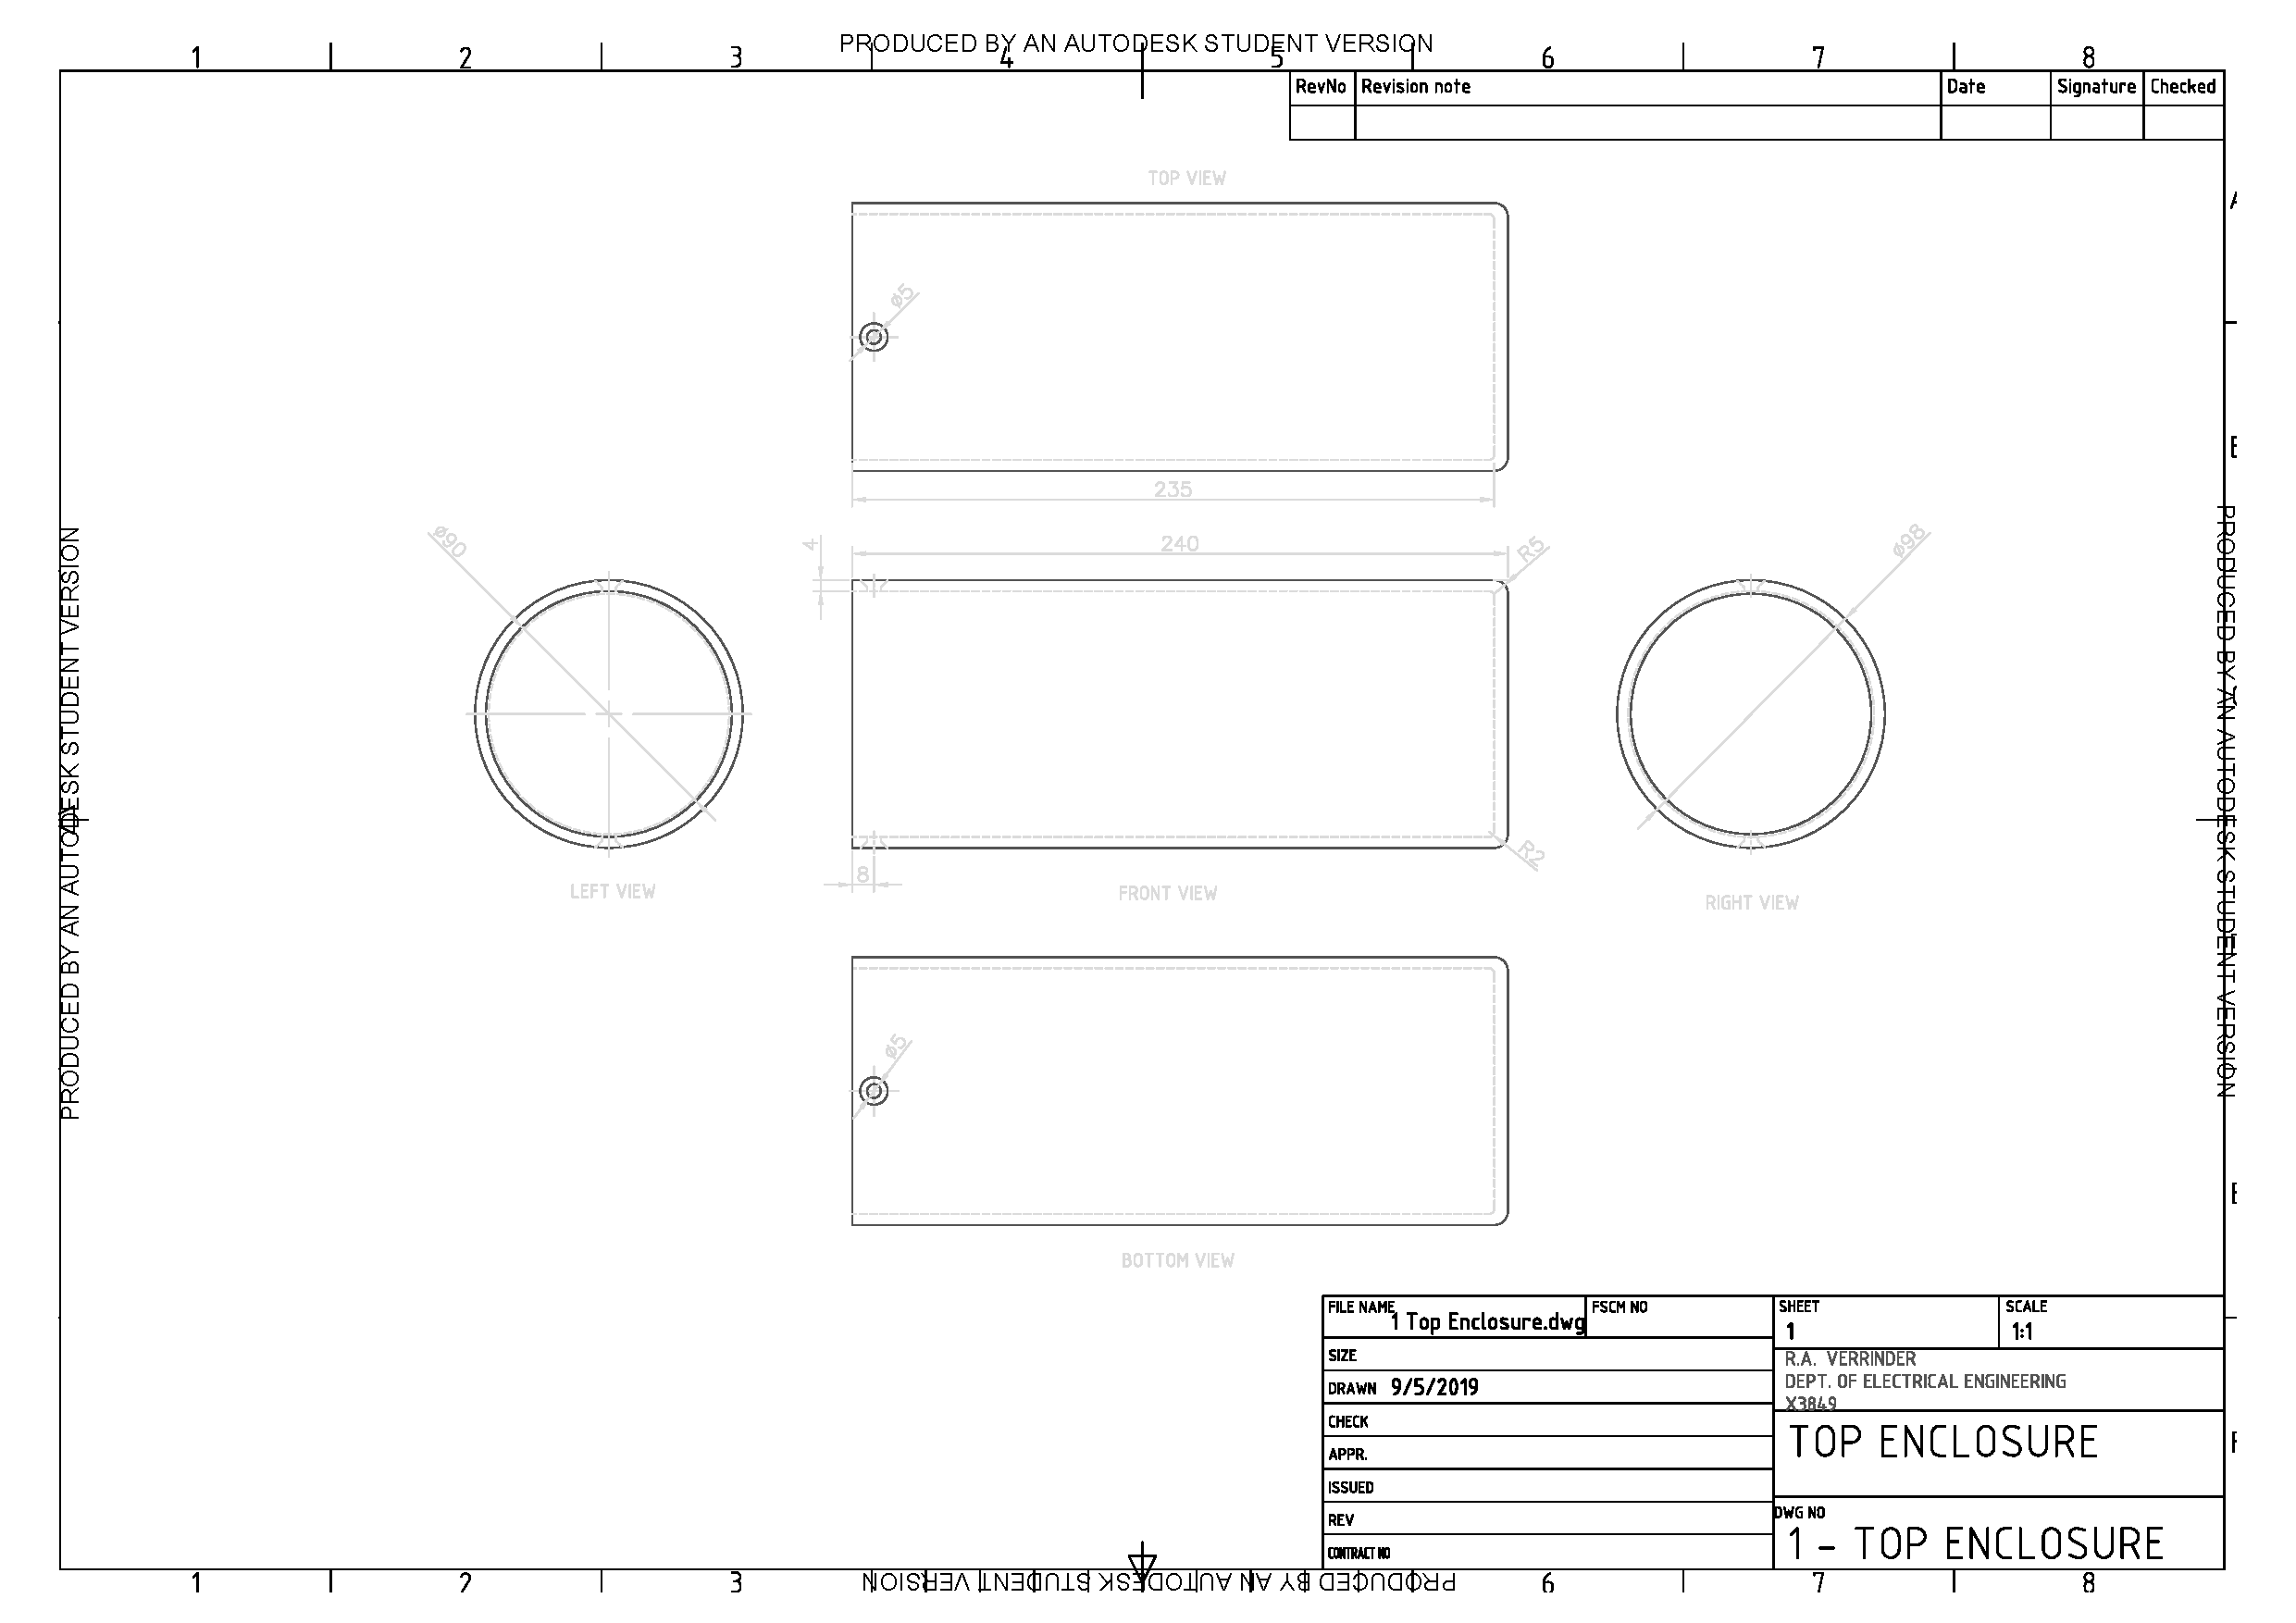
\includegraphics[page= 1,width= 0.9\textwidth]{enclosure}
	\caption{Schematic of top enclosure which protects the electronics.}
	\label{fig:top_schem}
\end{figure}

\begin{figure}[H]
	\centering
	\includegraphics[page= 2,width= 0.9\textwidth]{enclosure}
	\caption{Schematic of bottom enclosure for the batteries and power system.}
	\label{fig:bot_schem}
\end{figure}

\begin{figure}[H]
	\centering
	\includegraphics[page= 3,width= 0.9\textwidth]{enclosure}
	\caption{Schematic of the connector block which provides a base for the electronics to be mounted on. }
	\label{fig:conblock_schem}
\end{figure}

\begin{figure}[H]
	\centering
	\includegraphics[page= 4,width= 0.9\textwidth]{enclosure}
	\caption{Full enclosure schematic.}
	\label{fig:full_schem}
\end{figure}

%Event/ Interrupt description
\chapter{Software design}

\section{Events and interrupt handling protocols} 
\label{sec:evt}

\begin{table}[H]
	\centering
	\caption{Description of interrupt generated by the Iridium module on an external digital input line.}
	\setlength{\extrarowheight}{5pt}
	\begin{tabular}{|>{\raggedright\arraybackslash}m{0.25\textwidth}|>{\raggedright\arraybackslash}m{0.75\textwidth}|}
		\hline
		\multicolumn{2}{|l|}{\textbf{Ring Indicator}} \\
		\hline
		\textbf{Entry condition}  &  Buoy in any state other than reset with GPIO mapped to EXTI, or with wake up from sleep mode on a wake up pin(WUP). The WUP pin receives a digital high from the ring indicator pin on Iridium\\
		\hline
		\textbf{Function} &  The user has transmitted a packet to the buoy. Download the packet and execute/store the data based on the packet structure.\\
		\hline
		\textbf{Entry condition} & Device has downloaded user data which has been used to update the system and store data.\\
		\hline
		\textbf{Return state}& If entry source was a wake up, device will return to sleep, otherwise device will return to the main loop.\\
		\hline
	\end{tabular}
	
	\label{tab:Int_desc_RI}
\end{table}

\begin{table}[H]
	\centering
	\caption{Description of routine for interrupts generated by the IMU on an external digital input line.}
	\setlength{\extrarowheight}{5pt}
	\begin{tabular}{|>{\raggedright\arraybackslash}m{0.25\textwidth}|>{\raggedright\arraybackslash}m{0.75\textwidth}|}
		\hline
		\multicolumn{2}{|l|}{\textbf{IMU motion event detection}} \\
		\hline
		\textbf{Entry condition}  & Buoy in any state other than reset with GPIO wake up pin mapped to an EXTI line, with wake up from sleep mode enabled. The WUP pin receives a digital high from an exteranl interrupt pin.\\
		\hline
		\textbf{Function} & Device reads the interrupt source from the IMU, initializes I$^2$C peripheral and begins sampling IMU data. The interrupt source determines the sampling rate, period and mode.\\
		\hline
		\textbf{Entry condition} & Device will exit when the IMU has finished sampling and the data has been stored into memory.\\
		\hline
		\textbf{Return state} & If entry source was a wake up, device will return to sleep, otherwise device will return to the main loop.\\
		\hline
	\end{tabular}
	
	\label{tab:Int_desc_IMU}
\end{table}

\begin{table}[H]
	\centering
	\caption{Description of event handling routine for a brown out recovery event.}
	\setlength{\extrarowheight}{5pt}
	\begin{tabular}{|>{\raggedright\arraybackslash}m{0.25\textwidth}|>{\raggedright\arraybackslash}m{0.75\textwidth}|}
		\hline
		\multicolumn{2}{|l|}{\textbf{Brown out detection}} \\
		\hline
		\textbf{Entry condition}  & Buoy is in run mode or in standby mode with brown out detection voltage enabled and $V_{brownout}$ configured in option bytes. The event occurs when the voltage supplied to the microcontroller is less than $V_{brownout}$  causing the device to be held under reset. When the voltage rises above the threshold, the device will enter the handler. \\
		\hline
		\textbf{Function} & Device resets the relevant register flags and checks for data corruption. If no data is corrupted. Device will reload the last state and attempt to run it again. Otherwise the device performs a software reset \\
		\hline
		\textbf{Entry condition} & $V_{supply} > V_{brownout}$, device successfully executes code in handler. \\
		\hline
		\textbf{Return state} & Returns to main loop.\\
		\hline
	\end{tabular}
	\label{tab:Ev_desc_BoD}
\end{table}

\begin{table}[H]
	\centering
	\caption{Description of routine for handling low power events.}
	\setlength{\extrarowheight}{5pt}
	\begin{tabular}{|>{\raggedright\arraybackslash}m{0.25\textwidth}|>{\raggedright\arraybackslash}m{0.75\textwidth}|}
		\hline
		\multicolumn{2}{|l|}{\textbf{Low power detection}} \\
		\hline
		\textbf{Entry condition}  & Device is in run or sleep, the power voltage thresholds are set in PWR and the low power interrupt is enabled. The event occurs when $V_{supply} < V_{power}$ generating an event interrupt. \\
		\hline
		\textbf{Function} & Device will read the current sensor and transmit a final packet to the user. All peripherals switched off, and the device is turned off.\\
		\hline
		\textbf{Entry condition} & No exit.\\
		\hline
		\textbf{Return state} & No return state.\\
		\hline
	\end{tabular}
	
	\label{tab:Ev_desc_LPD}
\end{table}

\begin{table}[H]
	\centering
	\caption{Description of routine for handling a software reset event.}
	\setlength{\extrarowheight}{5pt}
	\begin{tabular}{|>{\raggedright\arraybackslash}m{0.25\textwidth}|>{\raggedright\arraybackslash}m{0.75\textwidth}|}
		\hline
		\multicolumn{2}{|l|}{\textbf{Software reset}} \\
		\hline
		\textbf{Entry condition}  & The Microcontroller reset line is pulled low for a few seconds. This is triggered in any state by triggering a software reset in the NVIC.\\
		\hline
		\textbf{Function} & Reset the buoy to an initial state, Clear any pending flags and reset system data in the RTC back up registers.\\
		\hline
		\textbf{Entry condition} & Successful reset of voltage domains.\\
		\hline
		\textbf{Return state} & Return to reset state and start of main loop.\\
		\hline
	\end{tabular}
	
	\label{tab:Ev_desc_SWR}
\end{table}


\section{Initialization Routines}

\begin{table}[H]
	\centering
	\caption{Colour guide for the initialization routine flow diagrams.}
	\begin{tabular}{l}
		\hline
		\cellcolor{micro}Microcontroller (HAL) function \\
		\cellcolor{sensor}Sensor (API) function \\
		\cellcolor{conditional}Function return statement evaluation \\
		\cellcolor{wrong}Fail return status \\
		\cellcolor{succ}Success return status\\
		\hline
	\end{tabular}
	
	\label{tab:Init_routine_Guide}
\end{table}


\begin{figure}[H]
	\centering
	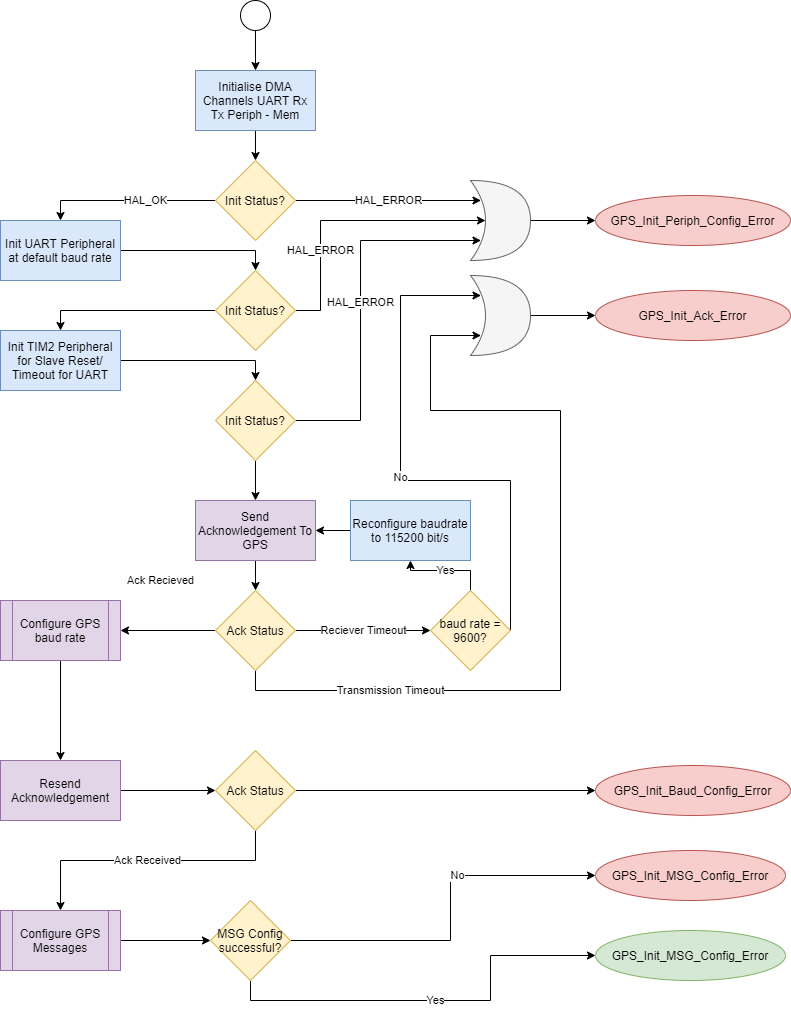
\includegraphics[scale=0.3]{GPS Initialization Algorithm .png}
	\caption{u-blox NEO-7M and u-blox NEO-M9N initialisation routine.}
	\label{fig:Init_diagram_gps}
\end{figure}

\begin{figure}[H]
	\centering
	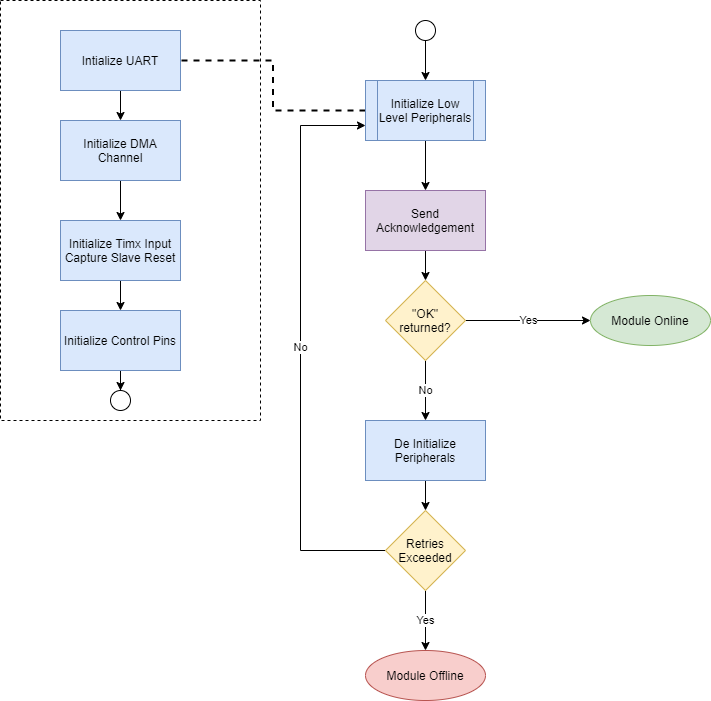
\includegraphics[scale=0.3]{Iridium Init Routine.png}
	\caption{Rock Seven RockBLOCK 9603 initialisation routine.}
	\label{fig:Init_diagram_ir}
\end{figure}


\begin{figure}[H]
	\centering
	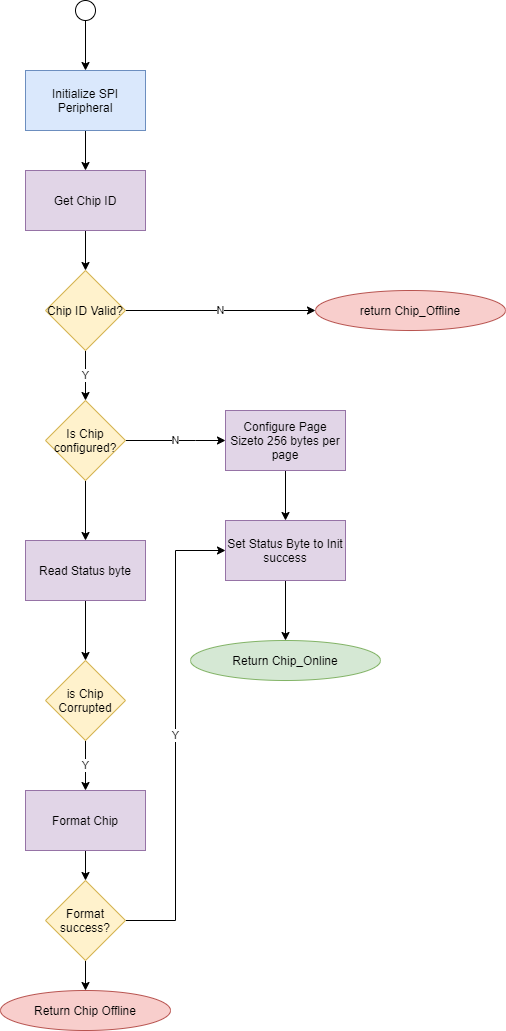
\includegraphics[scale=0.3]{Flash Chip Init Routine.png}
	\caption{Adesto Technologies AT45DB641E initialisation routine.}
	\label{fig:Init_diagram_flash}
\end{figure}

\begin{figure}[H]
	\centering
	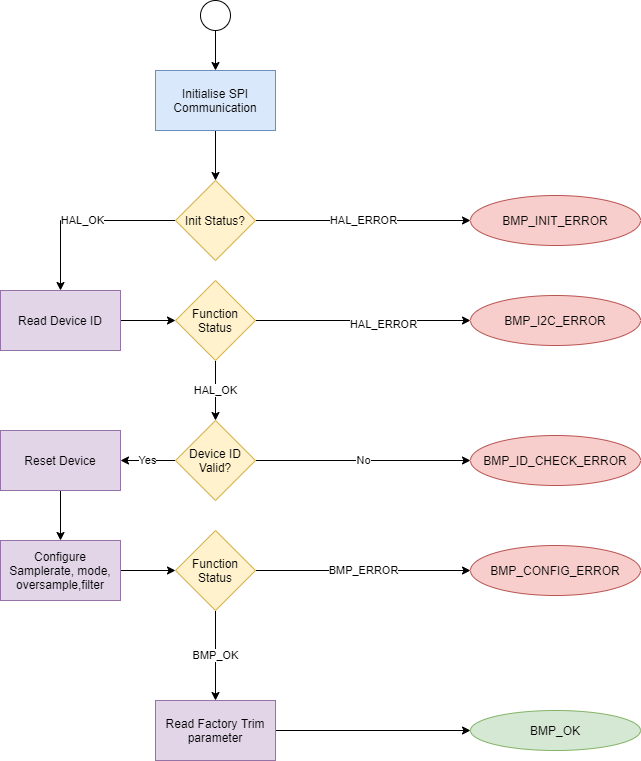
\includegraphics[scale=0.3]{Environmental Sensor Init Routine.png}
	\caption{Bosch Sensortech BMP280 initialisation routine.}
	\label{fig:Init_diagram_bmp}
\end{figure}

\begin{figure}[H]
	\centering
	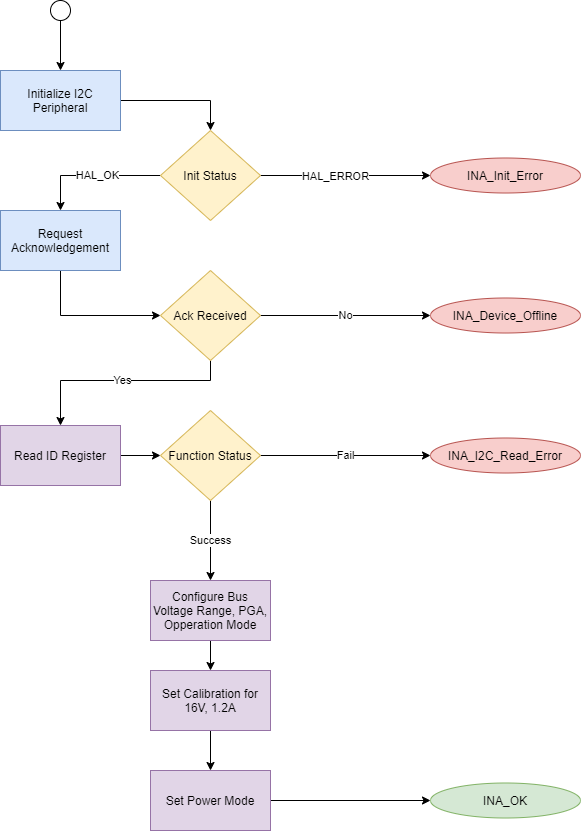
\includegraphics[scale=0.3]{INA219 Init routine.png}
	\caption{Texas Instruments INA219 initialisation routine.}
	\label{fig:Init_diagram_ina}
\end{figure}

\begin{figure}[H]
	\centering
	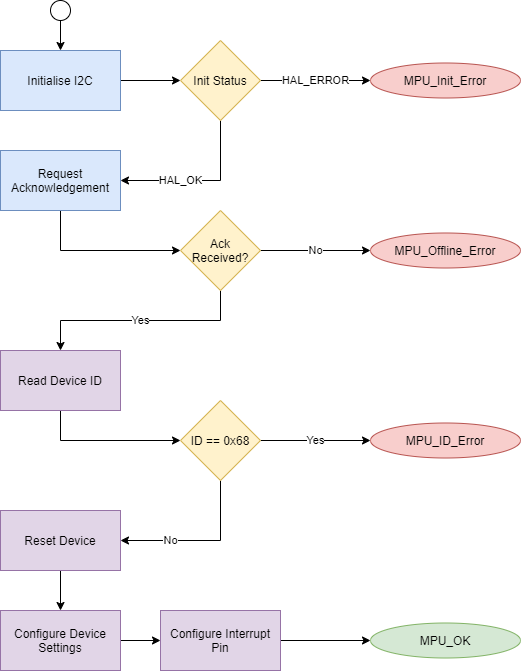
\includegraphics[scale=0.3]{MPU Init Diagram.png}
	\caption{TDK Invensense MPU6050 initialization routine.}
	\label{fig:Init_diagram_mpu}
\end{figure}

\section{Code}

\subsection{BMP280 temperature compensation formula}
\begin{figure}[H]
	
	\begin{lstlisting}
		/*
		* @brief Temperature Compensation algorithm
		*
		* @param T_val
		* @param t_fine
		* @param bmp_trim
		*
		* @retval int32_t
		*/
		int32_t BMP280_Compensate_Temp(int32_t T_val,int32_t* t_fine, BMP280_trim_t bmp_trim)
		{
			//compensate Temperature from datasheet
			int32_t var1 = (((T_val>>3)- ((int32_t)bmp_trim.dig_T1<<1))*((int32_t)bmp_trim.dig_T2))>>11;
			int32_t var2 =  (((((T_val>>4) - ((int32_t)bmp_trim.dig_T1)) * ((T_val>>4) - ((int32_t)bmp_trim.dig_T1))) >> 12)*((int32_t)bmp_trim.dig_T3)) >> 14;
			int32_t temp = var1+var2; //for storage in global variable
			*t_fine = temp;
			return (temp*5 +128)/256;
		}
		
	\end{lstlisting}
	\caption{Function written to compensate  a 32 bit Temperature reading for sensor irregularities using the 32 bit version of the recommended compensation formula from the datasheet \cite{BMP280_Datasheet}. The formula uses the compensation parameters stored on the sensor}
	\label{fig:bmp_code_comp_T}
\end{figure}

\begin{figure}[H]
	\begin{lstlisting}
		/*
		* @brief Pressure compensation formula
		*
		* @param P_val
		* @param t_fine
		* @param bmp_trim
		*
		* @retval uint32_t
		*/
		uint32_t BMP280_Compensate_Pressure(uint32_t P_val,int32_t t_fine,BMP280_trim_t bmp_trim)
		{
			//Compensation formula
			int32_t var1 = (int64_t)t_fine - 128000;
			int64_t var2 = var1*var1*((int64_t)(bmp_trim.dig_P6));
			var2 = var2 + (((int64_t)bmp_trim.dig_P4)<<35);
			var1 = ((var1 * var1 * (int64_t)bmp_trim.dig_P3)>>8) + ((var1 * (int64_t)bmp_trim.dig_P2)<<12);
			var1 = (((((int64_t)1)<<47)+var1))*((int64_t)bmp_trim.dig_P1)>>33;
			//check for divide by 0 error
			if(var1 == 0)return 0;
			int64_t P = 1048576 - (int32_t)P_val;
			P = (((P<<31)-var2)*3125)/var1;
			var1 = (((int64_t)(bmp_trim.dig_P9)) * (P>>13) * (P>>13)) >> 25;
			var2 = (((int64_t)(bmp_trim.dig_P8)) * P) >> 19;
			P = ((P + var1 + var2) >> 8) + (((int64_t)(bmp_trim.dig_P7))<<4);
			return (uint32_t)P;
		}
		
	\end{lstlisting}
	\caption{Function written to compensate  a 32-bit pressure reading for sensor irregularities using the 32-bit version of the recommended compensation formula from \cite{BMP280_Datasheet}. The formula uses the factory trim compensation parameters stored on the sensor.}
	\label{fig:bmp_code_comp_P}
\end{figure}

\subsection{INA219 calibration algorithm}
\begin{lstlisting}[breaklines=true]
	/*
	* Function Name INA_Status_t INA219_Calibrate_16V_1_2A(float *I_MBO, float *V_MBO, float *P_Max)
	* @brief: The following function writes a 16 bit value to the calibration register which
	* 			is used to adjust the current, bias voltage and power. Here, A LSB value is
	* 			calculated based on the user requirements and selected from a range. It would
	* 			be advisable to calculate the value manually and replace it in the function below
	* 			please note: the following function has values calculated manually. These can be
	* 			changed based on the configuration settings.
	* 			The values are calculated for 16V bus voltage range with a 2A expected current and
	* 			a 160mV shunt voltage range
	*
	* 	Step 1: V_Bus_Max = 16V
	* 			V_Shunt_Max = 160mV
	* 			R_Shunt = 0.1 Ohm
	*
	* 	Step 2: Max Possible I = 1.6A
	*
	* 	Step 3: Let I Max Expected = 1.2A
	*
	* 	Step 4: Min LSB = 36.6 uA/LSB
	* 			Max LSB = 292.97 uA
	*
	* 			Choose LSB = 100 uA
	* 	Step 5: Set Calibration value = 4096
	*/
	
	INA_Status_t INA219_Calibrate_16V_1_2A(float *I_MBO, float *V_MBO, float *P_Max)
	{
		//set Current Step Size
		ina.INA219_I_LSB = 100.0/1000000.0;
		uint16_t I_cal_val = (uint16_t)(0.04096/(ina.INA219_I_LSB*INA219_R_SHUNT));
		ina.INA219_P_LSB = 20*ina.INA219_I_LSB;
		float I_max = ina.INA219_I_LSB*32767;
		if(I_max  > 1.6) //max possible current
		{
			*I_MBO = 1.6;
		}else
		{
			*I_MBO = I_max;
		}
		float Vshunt_max = *I_MBO*INA219_R_SHUNT;
		if(Vshunt_max > 0.16)
		{
			*V_MBO = 0.16;
		}
		else
		{
			*V_MBO = Vshunt_max;
		}
		*P_Max = *I_MBO*16;
		
		//write I_Cal_val to register
		uint8_t temp[2] = {(I_cal_val&0xFF00)>>8,(I_cal_val&0x00FF)};
		if(HAL_I2C_Mem_Write(&ina.ina_i2c,INA219_I2C_Address,CALIBRATION_REG,1,temp,2,100) != HAL_OK)
		{
			return INA_I2C_WRITE_ERROR;
		}
		
		return INA_OK;
	}
	
\end{lstlisting}
\begin{center}
	\captionsetup{type=figure}
	\captionof{figure}{Calibration routine for INA219 current sensor for a maximum current of 1.2 A, maximum bus voltage of 16 V and maximum shunt voltage of 160 mV.}
	\label{fig:INA_Calib}
\end{center}

\subsection{Data structs}
\begin{figure}[H]
	\centering
	\begin{lstlisting}
		/*
		* Coordinate Object
		*
		* Stores the Cordinates of GPS in the form DDMM.mmmm
		* where 
		*          DD     -   Degrees
		*          MM     -   Minutes
		*          mmmm   -   Fractional minutes
		* Variables:	Name.............Type.................................Description
		* 				lat..............float32_t............................GPS Lattitude
		* 				longi............float32_t............................GPS Longitude
		*/
		typedef struct
		{
			float_t lat;
			float_t longi;
		}Coord_t;
	\end{lstlisting}    
	\caption{Coord\_t data structure to store incoming GPS coordinates as IEEE754 32-bit floats.}
	\label{fig:data_coord_t}
\end{figure}

\begin{figure}[H]
	\centering
	\begin{lstlisting}
		/*
		* Diagnostic Object
		*
		* Structure to Hold the GPS data signal diagnostics
		*
		* Variables:	Name.............Type.................................Description
		* 				PDOP.............DOP_t................................Positional dilution of Precision (3D)
		* 				HDOP.............DOP_t................................Horizontal dilution of Precision
		* 				VDOP.............DOP_t................................Vertical   dilution of Precision
		* 				num_sats.........uint8_t..............................Number of Satelites used to obtain positional Fix
		* 				fix_type.........uint8_t..............................number between 1-3 describing the type of fix obtained
		*
		* Fix types
		* 1 - No Fix
		* 2 - 2D Fix (No altitude)
		* 3 - 3D Fix
		*/
		
		typedef struct
		{
			DOP_t PDOP;
			DOP_t HDOP;
			DOP_t VDOP;
			uint8_t num_sats;
			uint8_t fix_type;
		}Diagnostic_t;
	\end{lstlisting}
	\caption{Data structure for storing GPS signal diagnostic information.}
	\label{fig:data_Diagnostic_t}
\end{figure}


\chapter{Supplementary tables}

\begin{table}[H]
	\centering
	\caption{List of data services provided by Iridium for transmission of data over the satellite network including the bandwidth and purpose of the service taken from \cite{iridium_mobile}.}
	\label{tab:iridium service}
	\setlength{\extrarowheight}{5pt}
	\resizebox{\textwidth}{!}{%
	\begin{tabular}{>{\RaggedRight}m{0.3\textwidth}>{\raggedright\arraybackslash}m{0.4\textwidth}>{\raggedright\arraybackslash}m{0.3\textwidth} >{\raggedright\arraybackslash}m{0.3\textwidth}}
		\hline
		\textbf{Service name} & \textbf{Purpose}& \textbf{Supporting modems} & \textbf{Bandwidth}\\
		\hline
		\hline
		\multirow{3}{*}{Short Burst Data (SBD)} & \multirow{3}{*}{Sending short messages in bursts.} &  9603/9602 & 340 bytes upload \& 270 bytes download \\
			&&9523 & 1960 bytes upload \& 1890 bytes download\\
			&& Iridium edge &\\
		\hline
		\multirow{2}{0.3\textwidth}{Router-based Unrestricted Digital Interworking Connectivity Solution (RUDICS)} & 	\multirow{2}{0.4\textwidth}{Continuous transfer of large real-time data from a large array of devices to a host.} & 9523  & \multirow{2}{0.3\textwidth}{6 to 10 KB/min}\\
			&& 9522B \par (\textit{depreciated})&\\
		\hline
		\multirow{2}{0.3\textwidth}{Circuit Switch Data (CSD)} & 	\multirow{2}{0.4\textwidth}{ Continuous transmission of large volumes of data over a dial-Up network using a SIM card.} & 9523  & \multirow{2}{0.3\textwidth}{6 to 10 KB/min}\\
		&& 9522B \par (\textit{depreciated})&\\
		\hline
		\hline
	\end{tabular}}
\end{table}

\newpage
\begin{table}[H]
		\centering
		\caption{Strategies used by the devices to transfer data from remote locations. Table includes transmission technologies and services used as well and transmission strategies and transmission intervals where given. Prices are converted to Rands (R) via \cite{usdcoversion}.}
		\label{tab:device_transmissionstrategies}
		\setlength{\extrarowheight}{5pt}%
		\resizebox{\textwidth}{!}{%
		\begin{tabular}{>{\RaggedRight}m{4cm} >{\RaggedRight}m{4cm} >{\RaggedRight}m{3cm} >{\RaggedRight}m{4cm} >{\RaggedRight}m{6cm}}
			\hline
			\textbf{Device name}  & \textbf{Service} & \textbf{Modem} & \textbf{Bandwidth} & \textbf{Transmission strategy}\\
			\hline
			\hline
			WIIB  & Iridium SBD & 9602 & 340 bytes &  Data condensed into one 340 byte packet (transmission intervals unavailable).\\
			\hline
			WIIOS & Iridium SBD & 9602 & 340 bytes & Data condensed into one 340 byte packet transmitted every five hours. \\
			\hline
			NDWB & Iridium RUDICS & 9522B & 6 to 10 KB/min & Raw IMU data points transmitted every minute.\\
			\hline
			\multirow{4}{4cm}{SKIB} & Iridium SBD (long range) & 9602 & 340 bytes & GPS data transmitted every 10 minutes. \\
			& ZigBee (short range)& Xbee Pro & 50 KB/second & Raw data transmitted when host is in range.\\
			\hline
				\multirow{6}{2cm}{SWIFT} &  Iridium & Geoforce SmartOne (tracking) & N/A & Not Reported/\\
				& Iridium SBD & Unspecified SBD Modem (telemetry) & 1960 bytes & Data transmitted through SBD modem. variable packet sizes ranging from 4 to 1228 bytes in length.\\
				& Ethernet & Digi Xpress ethernet bridge  & 935 KB/second & Not Reported.\\
			\hline
			\multirow{2}{4cm}{SIMB} & Iridium &9603 &340 bytes &Single packet transmission of 275 bytes.\\
			& ARGOS & Not Reported & Not Reported & Not Reported \\
			\hline
			Polar ISVP & Iridium SBD& 9602 & 340 bytes & User configured packet sizes and transmission intervals.\\
			\hline
			Trident & Iridium SBD& 9603 & 340 bytes & Single packet transmission of 16 bytes. \\
			\hline
			\hline
	\end{tabular}}

\end{table}
\newpage

\chapter{Test protocols}

\section{Unit tests}
\label{app:Unittests}
\begin{table}[H]
	\centering
	\setlength{\extrarowheight}{5pt}
	\caption{ Protocol for firmware initialisation/deinitialisation functional test.}
	\label{tab:UT001}
	\begin{tabular}{m{0.2\textwidth} m{0.7\textwidth}}
		\multicolumn{2}{l}{\textbf{UT001} }\\
		\hline
		\textbf{Description} & Initialisation/deinitialisation test.\\
		\hline
		\hline
		\textbf{Test protocol} & The hardware module is connected to the microcontroller with the corresponding subsystem API libraries and driver files. The initialisation/deinitialsation function is run. After the function has completed, the return status from the function is evaluated. If the test was completed sucessfully, A "Module online!" is printed to the serial and the LED is switched on. \\
		\hline
		\hline
	\end{tabular}
\end{table}

\begin{table}[H]
	\centering
	\caption{Protocol for the signal acquisition firmware test, This test is specific to receivers with wireless capabilities. }
	\setlength{\extrarowheight}{5pt}
	\label{tab:UT002}
	\begin{tabular}{m{0.2\textwidth} m{0.7\textwidth}}
		\multicolumn{2}{l}{\textbf{UT002} }\\
		\hline
		\textbf{Description} & Signal acquisition test.\\
		\hline
		\hline
		\textbf{Test protocol} & Test to be run after unit test UT001 in Table \ref{tab:UT001}. Module de initialisation function is to be run until completion. After the function has run, the configuration registers are checked for reset values. If the registers are reset, the function returns a success status and "Successfully deinitialised module!" is printed to the serial. If the LED was green, it is turned off. This test was also run before an initialisation function to ensure that the function does not result in hard faults.\\
		\hline
		\hline
	\end{tabular}
\end{table}

\begin{table}[H]
	\centering
	\caption{protocol for testing the peripheral communication functional unit. }
	\setlength{\extrarowheight}{5pt}
	\label{tab:UT003}
	\begin{tabular}{m{0.2\textwidth} m{0.7\textwidth}}
		\multicolumn{2}{l}{\textbf{UT003} }\\
		\hline
		\textbf{Description} & Signal acquisition test.\\
		\hline
		\hline
		\textbf{Test protocol} & Module to be connected to the microcontroller with firmware loaded with the required communication peripherals to be initialised. The microcontroller either requests to receive a byte of data or transmits a set of data in polling mode. If successful, the function will return a successful status. Otherwise am error code will be returned.\\
		\hline
		\hline
	\end{tabular}
\end{table}


\begin{table}[H]
	\centering
	\caption{Protocol for testing a software function for validating sensor data.}
	\label{tab:UT004}
		\setlength{\extrarowheight}{5pt}
	\begin{tabular}{m{0.2\textwidth} m{0.7\textwidth}}
		\multicolumn{2}{l}{\textbf{UT004} }\\
		\hline
		\textbf{Description} & Transmission test\\
		\hline
		\hline
		\textbf{Test protocol} & Test to be run as a unit test on the desired platform. An array of expected outputs from the sensor is written as a test case along with the expected output of the function. Then the input is passed through the function and stored after the function has been complete. The function output is compared to the expected output. The function passes if the output matches the expected output.    \\
		\hline
		\hline
	\end{tabular}
\end{table}

\begin{table}[H]
	\centering
	\caption{ Protocol for testing data streams and direct memory access (DMA) functions.}
	\label{tab:UT005}
	\setlength{\extrarowheight}{5pt}
	\begin{tabular}{m{0.2\textwidth} m{0.7\textwidth}}
		\multicolumn{2}{l}{\textbf{UT005} }\\
		\hline
		\textbf{Description} & Data stream test\\
		\hline
		\hline
		\textbf{Test protocol} & The hardware module is connected to the microcontroller with the DMA stream enabled. The microcontroller triggers the sensor to transmit a known amount of data through the DMA stream. The microcontroller waits for a signal to close the stream then stops the DMA transfer. The data from the stream is then compared to the data expected. The test fails immediately if errors or hard faults occur.\\
		\hline
		\hline
	\end{tabular}
\end{table}

\begin{table}[H]
	\centering
	\caption{ Protocol to test functions that interface with sensors by configuring settings in the register or reading data from a register.}
	\label{tab:UT006}
	\setlength{\extrarowheight}{5pt}
	\begin{tabular}{m{0.2\textwidth} m{0.7\textwidth}}
		\multicolumn{2}{l}{\textbf{UT006} }\\
		\hline
		\textbf{Description} & Sensor interface module functional test\\
		\hline
		\hline
		\textbf{Test protocol} & Test requires the module library to be loaded onto the microcontroller with the hardware module connected. Function to be called after a successful initialisation. Load the function with a known parameter and wait for a return status. Evaluate the return status against a table to determine whether the function was successful. \\
		\hline
		\hline
	\end{tabular}
\end{table}

\begin{table}[H]
	\centering
	\setlength{\extrarowheight}{5pt}
	\caption{ Protocols for fault testing of software subsystem functions.}
	\label{tab:UT007}
	\begin{tabular}{m{0.2\textwidth} m{0.7\textwidth}}
		\multicolumn{2}{l}{\textbf{UT007} }\\
		\hline
		\textbf{Description} & Unit fault testing\\
		\hline
		\hline
		\textbf{Test protocol} & Firmware to be loaded onto the microcontroller with the module placed in the configurations shown in AT002 (Table \ref{tab:AT002}). the test passes if each configuration results in the corresponding error code being returned. The test fails if the function freezes or does not return a predicatble return code.  \\
		\hline
		\hline
	\end{tabular}
\end{table}

\begin{table}[H]
	\centering
	\setlength{\extrarowheight}{5pt}
	\caption{ Protocols for testing digital input/output peripheral functional units.}
	\label{tab:UT008}
	\begin{tabular}{m{0.2\textwidth} m{0.7\textwidth}}
		\multicolumn{2}{l}{\textbf{UT007} }\\
		\hline
		\textbf{Description} & GPIO functional unit tests\\
		\hline
		\hline
		\textbf{Test protocol} & Firmware to be loaded onto the microcontroller with an LED attached to the digital pin. Pin to be configured in digital output mode. A logic high must be written to the pin resulting in a pass if the LED turns on. Then a logic low is written resulting in a pass if the LED turns off. For input testing, a push button in normally open mode must be attached to the pin and configured in pull up mode. A logic high should be read while the button is open and a logic low should be read while the button is pressed. \\
		\hline
		\hline
	\end{tabular}
\end{table}
\section{System test results}
\begin{table}[H]
	\centering
	\caption{Results of subsystem acceptance tests for each of the identified modules. Modules that were successfully validated were marked with a \checkmark, failed tests were marked by an X and tests that could not be applied to a subsystem were marked by an N/A.}
	\begin{tabular}{|c|c|c|c|c|c|}
		\cline{2-6}
		\multicolumn{1}{c|}{}&\textbf{AT001}&\textbf{AT002}&\textbf{AT003}&\textbf{AT004 }&\textbf{AT005 }\\
		\hline
		GPS &  \checkmark & \checkmark & \checkmark & \checkmark & \checkmark\\
		\hline
		Iridium Modem &  \checkmark & \checkmark & \checkmark & \checkmark & \checkmark\\
		\hline
		Flash Chips &  \checkmark & \checkmark & \checkmark & \checkmark &
		\checkmark\\ 
		\hline
		Power Module & N/A & N/A & \checkmark & N/A& N/A\\
		\hline
		Env Sensor  &  \checkmark & \checkmark & \checkmark & \checkmark &
		\checkmark\\
		\hline
		Power Monitor   &  \checkmark & \checkmark & \checkmark & \checkmark &
		\checkmark\\
		\hline
		IMU   &  \checkmark & \checkmark & \checkmark & \checkmark &
		\checkmark\\
		\hline
	\end{tabular}
	
	\label{tab:AT_SSYS_EV}
\end{table}
